
\section{Séance 3}

\vspace*{1cm}

\begin{exo}
Construisez un code de Gray d'ordre $5$ sur base du code de Gray d'ordre $4$ ci-dessous.\\
0000,0100,1100,1000,1010,1110,0110,0010,0011,0111,1111,1011,1001,1101,0101,0001
\end{exo}

\vspace*{1cm}

\begin{exo}
Dans le graphe ci-dessous, on donne un couplage de cardinal maximal. En utilisant la preuve du th\'eor\`eme de K\"onig vue au cours, trouvez un transversal de cardinal minimal.
\end{exo}

\begin{figure}[!h]
\begin{center}
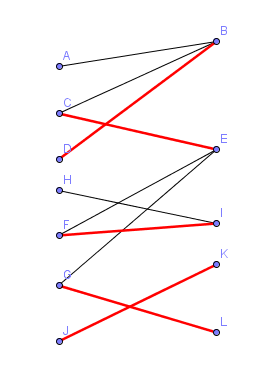
\includegraphics{../Figures/Transversal.png} 
\end{center}
\end{figure}

\begin{exo}
Sur $\R^2$, on d\'efinit les relations suivantes:
$$(x,y)\mathcal{R}(x',y') \Leftrightarrow x \leq x' \mathrm{~et~} y \leq y', $$
$$(x,y)\mathcal{S}(x',y') \Leftrightarrow (x < x') \mathrm{~ou~} (x = x' \mathrm{~et~} y \leq y').$$
Est-ce que les relations $\mathcal{R}$ et $\mathcal{S}$ sont des ordres?
\end{exo}

\newpage
\begin{exo}
Consid\'erons le graphe biparti (bipartition donn\'ee par une coloration des sommets) ci-dessous. Sur l'ensemble de ses sommets, on d\'efinit la relation $u\leq v$ pour $u,v$ des sommets tels que $u$ est un sommet rouge et $\{u,v\}$ est une ar\^ete. On pose aussi $u\leq u$ pour tout sommet $u$. \\
\begin{enumerate}[(a)]
\item V\'erifiez que $\leq$ est un ordre partiel.
\item Construisez une partition des sommets par $k$ cha\^ines et trouvez une anticha\^ine contenant $k$ \'el\'ements.
\item D\'eduisez-en un couplage de cardinalit\'e maximale et un transversal de cardinalit\'e minimale. 
\item (Bonus) Sur base de ce qui est fait ci-dessus, prouvez que le th\'eor\`eme de K\"onig implique le th\'eor\`eme de Dilworth.
\end{enumerate}
\end{exo}

\begin{figure}[!h]
\begin{center}
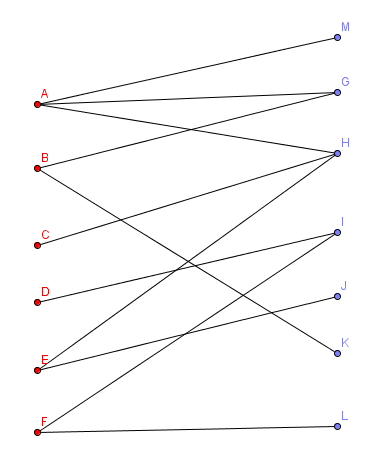
\includegraphics{../Figures/Konig.png} 
\end{center}
\end{figure}